% Options for packages loaded elsewhere
\PassOptionsToPackage{unicode}{hyperref}
\PassOptionsToPackage{hyphens}{url}
\PassOptionsToPackage{dvipsnames,svgnames,x11names}{xcolor}
%
\documentclass[
]{article}

\usepackage{amsmath,amssymb}
\usepackage{lmodern}
\usepackage{iftex}
\ifPDFTeX
  \usepackage[T1]{fontenc}
  \usepackage[utf8]{inputenc}
  \usepackage{textcomp} % provide euro and other symbols
\else % if luatex or xetex
  \usepackage{unicode-math}
  \defaultfontfeatures{Scale=MatchLowercase}
  \defaultfontfeatures[\rmfamily]{Ligatures=TeX,Scale=1}
  \setmainfont[]{MINIONPRO-REGULAR.OTF}
  \setsansfont[]{MORISTONPERSONAL-REGULAR.OTF}
\fi
% Use upquote if available, for straight quotes in verbatim environments
\IfFileExists{upquote.sty}{\usepackage{upquote}}{}
\IfFileExists{microtype.sty}{% use microtype if available
  \usepackage[]{microtype}
  \UseMicrotypeSet[protrusion]{basicmath} % disable protrusion for tt fonts
}{}
\makeatletter
\@ifundefined{KOMAClassName}{% if non-KOMA class
  \IfFileExists{parskip.sty}{%
    \usepackage{parskip}
  }{% else
    \setlength{\parindent}{0pt}
    \setlength{\parskip}{6pt plus 2pt minus 1pt}}
}{% if KOMA class
  \KOMAoptions{parskip=half}}
\makeatother
\usepackage{xcolor}
\setlength{\emergencystretch}{3em} % prevent overfull lines
\setcounter{secnumdepth}{5}
% Make \paragraph and \subparagraph free-standing
\ifx\paragraph\undefined\else
  \let\oldparagraph\paragraph
  \renewcommand{\paragraph}[1]{\oldparagraph{#1}\mbox{}}
\fi
\ifx\subparagraph\undefined\else
  \let\oldsubparagraph\subparagraph
  \renewcommand{\subparagraph}[1]{\oldsubparagraph{#1}\mbox{}}
\fi


\providecommand{\tightlist}{%
  \setlength{\itemsep}{0pt}\setlength{\parskip}{0pt}}\usepackage{longtable,booktabs,array}
\usepackage{calc} % for calculating minipage widths
% Correct order of tables after \paragraph or \subparagraph
\usepackage{etoolbox}
\makeatletter
\patchcmd\longtable{\par}{\if@noskipsec\mbox{}\fi\par}{}{}
\makeatother
% Allow footnotes in longtable head/foot
\IfFileExists{footnotehyper.sty}{\usepackage{footnotehyper}}{\usepackage{footnote}}
\makesavenoteenv{longtable}
\usepackage{graphicx}
\makeatletter
\def\maxwidth{\ifdim\Gin@nat@width>\linewidth\linewidth\else\Gin@nat@width\fi}
\def\maxheight{\ifdim\Gin@nat@height>\textheight\textheight\else\Gin@nat@height\fi}
\makeatother
% Scale images if necessary, so that they will not overflow the page
% margins by default, and it is still possible to overwrite the defaults
% using explicit options in \includegraphics[width, height, ...]{}
\setkeys{Gin}{width=\maxwidth,height=\maxheight,keepaspectratio}
% Set default figure placement to htbp
\makeatletter
\def\fps@figure{htbp}
\makeatother
\newlength{\cslhangindent}
\setlength{\cslhangindent}{1.5em}
\newlength{\csllabelwidth}
\setlength{\csllabelwidth}{3em}
\newlength{\cslentryspacingunit} % times entry-spacing
\setlength{\cslentryspacingunit}{\parskip}
\newenvironment{CSLReferences}[2] % #1 hanging-ident, #2 entry spacing
 {% don't indent paragraphs
  \setlength{\parindent}{0pt}
  % turn on hanging indent if param 1 is 1
  \ifodd #1
  \let\oldpar\par
  \def\par{\hangindent=\cslhangindent\oldpar}
  \fi
  % set entry spacing
  \setlength{\parskip}{#2\cslentryspacingunit}
 }%
 {}
\usepackage{calc}
\newcommand{\CSLBlock}[1]{#1\hfill\break}
\newcommand{\CSLLeftMargin}[1]{\parbox[t]{\csllabelwidth}{#1}}
\newcommand{\CSLRightInline}[1]{\parbox[t]{\linewidth - \csllabelwidth}{#1}\break}
\newcommand{\CSLIndent}[1]{\hspace{\cslhangindent}#1}

\usepackage{flafter, amsmath, booktabs, caption, longtable, changepage, multirow}
\newenvironment{widestuff}{\begin{table}[h]\begin{adjustwidth}{-4.5cm}{-4.5cm}\centering}{\end{adjustwidth}\end{table}}
\makeatletter
\makeatother
\makeatletter
\makeatother
\makeatletter
\@ifpackageloaded{caption}{}{\usepackage{caption}}
\AtBeginDocument{%
\ifdefined\contentsname
  \renewcommand*\contentsname{Table of contents}
\else
  \newcommand\contentsname{Table of contents}
\fi
\ifdefined\listfigurename
  \renewcommand*\listfigurename{List of Figures}
\else
  \newcommand\listfigurename{List of Figures}
\fi
\ifdefined\listtablename
  \renewcommand*\listtablename{List of Tables}
\else
  \newcommand\listtablename{List of Tables}
\fi
\ifdefined\figurename
  \renewcommand*\figurename{Figure}
\else
  \newcommand\figurename{Figure}
\fi
\ifdefined\tablename
  \renewcommand*\tablename{Table}
\else
  \newcommand\tablename{Table}
\fi
}
\@ifpackageloaded{float}{}{\usepackage{float}}
\floatstyle{ruled}
\@ifundefined{c@chapter}{\newfloat{codelisting}{h}{lop}}{\newfloat{codelisting}{h}{lop}[chapter]}
\floatname{codelisting}{Listing}
\newcommand*\listoflistings{\listof{codelisting}{List of Listings}}
\makeatother
\makeatletter
\@ifpackageloaded{caption}{}{\usepackage{caption}}
\@ifpackageloaded{subcaption}{}{\usepackage{subcaption}}
\makeatother
\makeatletter
\@ifpackageloaded{tcolorbox}{}{\usepackage[many]{tcolorbox}}
\makeatother
\makeatletter
\@ifundefined{shadecolor}{\definecolor{shadecolor}{rgb}{.97, .97, .97}}
\makeatother
\makeatletter
\makeatother
\ifLuaTeX
  \usepackage{selnolig}  % disable illegal ligatures
\fi
\IfFileExists{bookmark.sty}{\usepackage{bookmark}}{\usepackage{hyperref}}
\IfFileExists{xurl.sty}{\usepackage{xurl}}{} % add URL line breaks if available
\urlstyle{same} % disable monospaced font for URLs
\hypersetup{
  pdftitle={Supporting Materials: Load Estimates},
  pdfauthor={Michael Schramm},
  colorlinks=true,
  linkcolor={blue},
  filecolor={Maroon},
  citecolor={Blue},
  urlcolor={Blue},
  pdfcreator={LaTeX via pandoc}}

\title{Supporting Materials: Load Estimates\thanks{This project was
funded by a Texas Coastal Management Program grant approved by the Texas
Land Commissioner, providing financial assistance under the Coastal Zone
Management Act of 1972, as amended, awarded by the National Oceanic and
Atmospheric Administration (NOAA), Office for Coastal Management,
pursuant to NOAA Award No.~NA21NOS4190136. The views expressed herein
are those of the author(s) and do not necessarily reflect the views of
NOAA, the U.S. Department of Commerce, or any of their subagencies.}}
\author{Michael Schramm}
\date{}

\begin{document}
\maketitle
\begin{abstract}
This document includes figures and tables summarizing total loading
estimates for the Lavaca River watershed.
\end{abstract}
\ifdefined\Shaded\renewenvironment{Shaded}{\begin{tcolorbox}[sharp corners, breakable, enhanced, interior hidden, boxrule=0pt, borderline west={3pt}{0pt}{shadecolor}, frame hidden]}{\end{tcolorbox}}\fi

\hypertarget{load-estimation-and-summarization}{%
\section{Load estimation and
summarization}\label{load-estimation-and-summarization}}

Daily Nitrate-Nitrogen (NO\textsubscript{3}-N) and Total Phosphorus (TP)
loads at stream sites were predicted using fitted GAM models. Standard
deviations and credible intervals from GAM models can be obtained by
drawing samples from the multivariate normal posterior distribution of
the fitted GAM (Wood 2006; Marra and Wood 2012; McDowell et al. 2021).
Uncertainty in loads were reported as 95\% credible intervals developed
by drawing 1000 realizations of parameter estimates from the
multivariate normal posterior distribution of the model parameters. We
re-estimated the load for each realization and report the 2.5\% and
97.5\% quantiles. Monthly and annual loads were calculated by summing
for each respective time period.

Daily flow variability is responsible for the majority of daily load
variability. WRTDS utilizes a flow- normalization procedure that removes
the influence of flow variability by treating daily flow as a random
sample of all possible discharges on a given day (Hirsch et al. 2010).
The flow-normalized estimates are not true estimates of load, but are
indicative of potential changes in load that are not attributable to
variability in daily flow. These flow-normalized estimates are most
suitable for assessing changes in long-term trends. We implemented a
similar procedure by setting flow-based covariates on each day of the
year equal to each of the historical values for that day of the year
between 2000 and 2021. The flow-normalized estimate is simply the mean
of the model predictions for each day considering all of the flow
values. Flow-normalized estimates and credible intervals were aggregated
to annual reporting periods following procedures used for predicted
actual loading.

\hypertarget{total-load-estimates}{%
\section{Total Load Estimates}\label{total-load-estimates}}

\hypertarget{lavaca-river-at-edna-usgs-08164000}{%
\subsection{Lavaca River at Edna,
USGS-08164000}\label{lavaca-river-at-edna-usgs-08164000}}

\begin{figure}[h]

{\centering 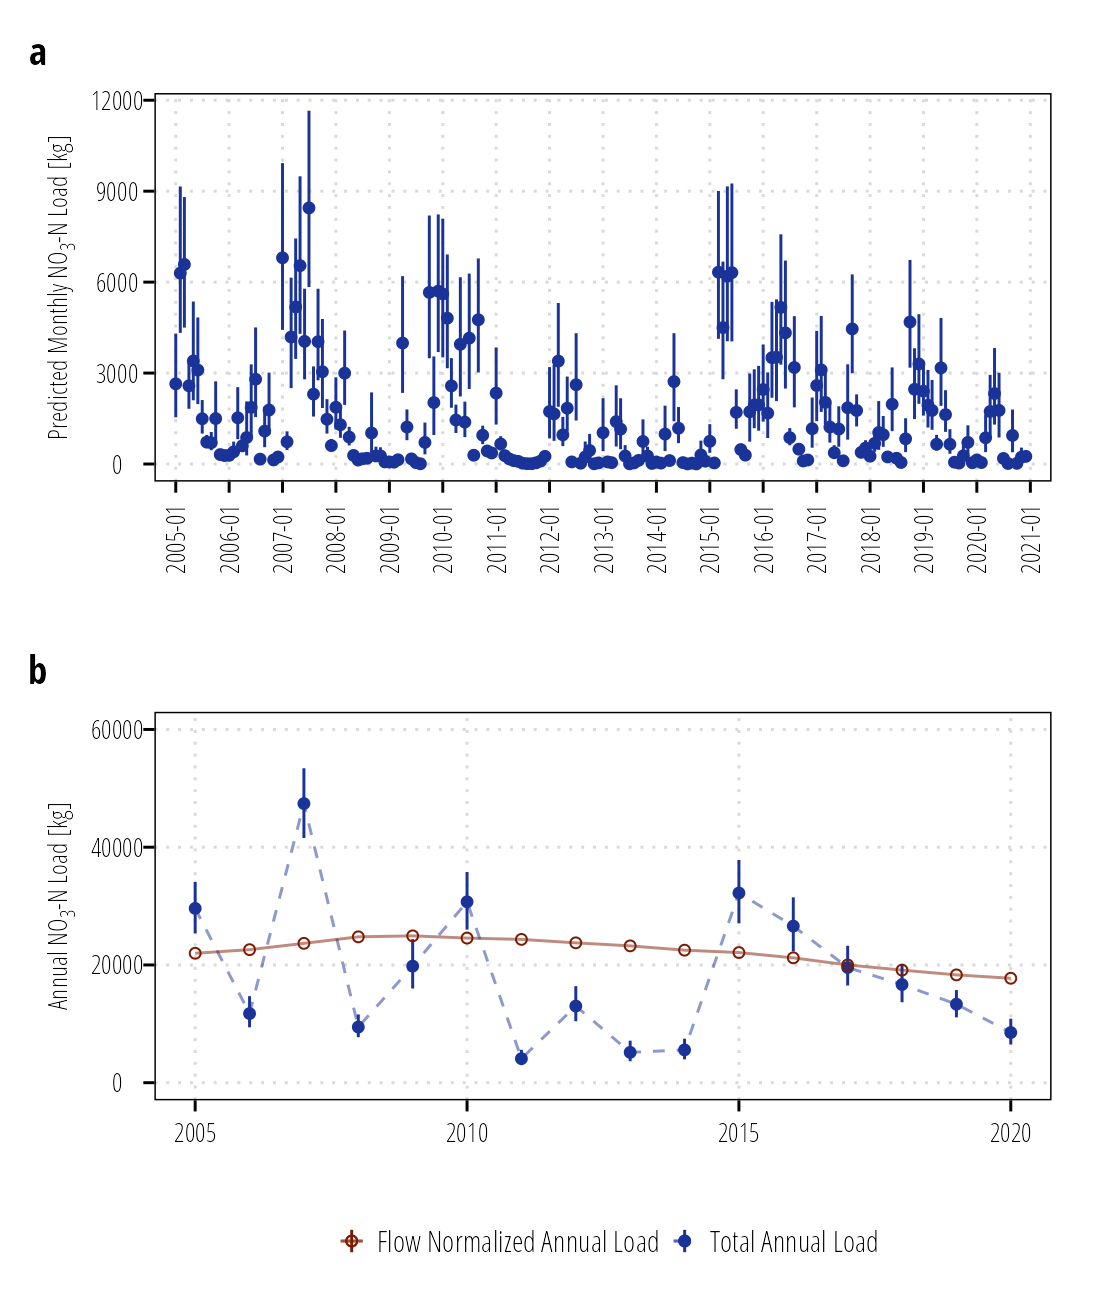
\includegraphics{load_estimates_files/figure-pdf/no3_aggregate-08164000-1.png}

}

\caption{Aggregated (a) monthly and (b) annual NO\textsubscript{3}-N
loads at Lavaca River at Edna, USGS-08164000.}

\end{figure}

\begin{figure}[h]

{\centering 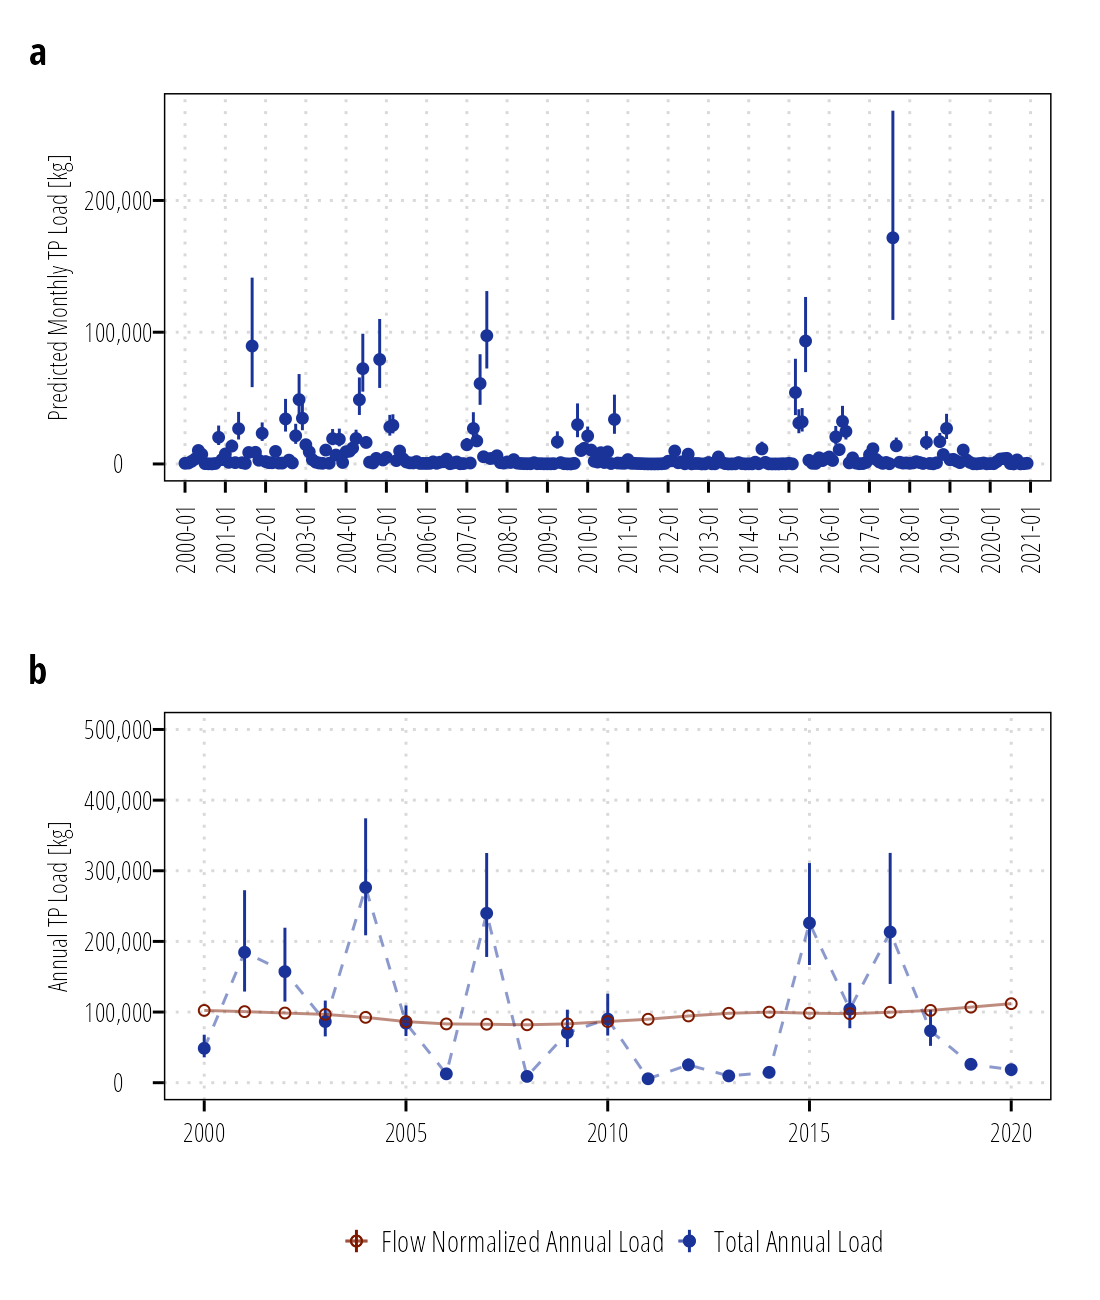
\includegraphics{load_estimates_files/figure-pdf/tp_aggregate-08164000-1.png}

}

\caption{Aggregated (a) monthly and (b) annual TP loads at Lavaca River
at Edna, USGS-08164000.}

\end{figure}

\clearpage

\hypertarget{navidad-river-at-palmetto-bend-dam-lake-texana}{%
\subsection{Navidad River at Palmetto Bend Dam, Lake
Texana}\label{navidad-river-at-palmetto-bend-dam-lake-texana}}

\begin{figure}[h]

{\centering 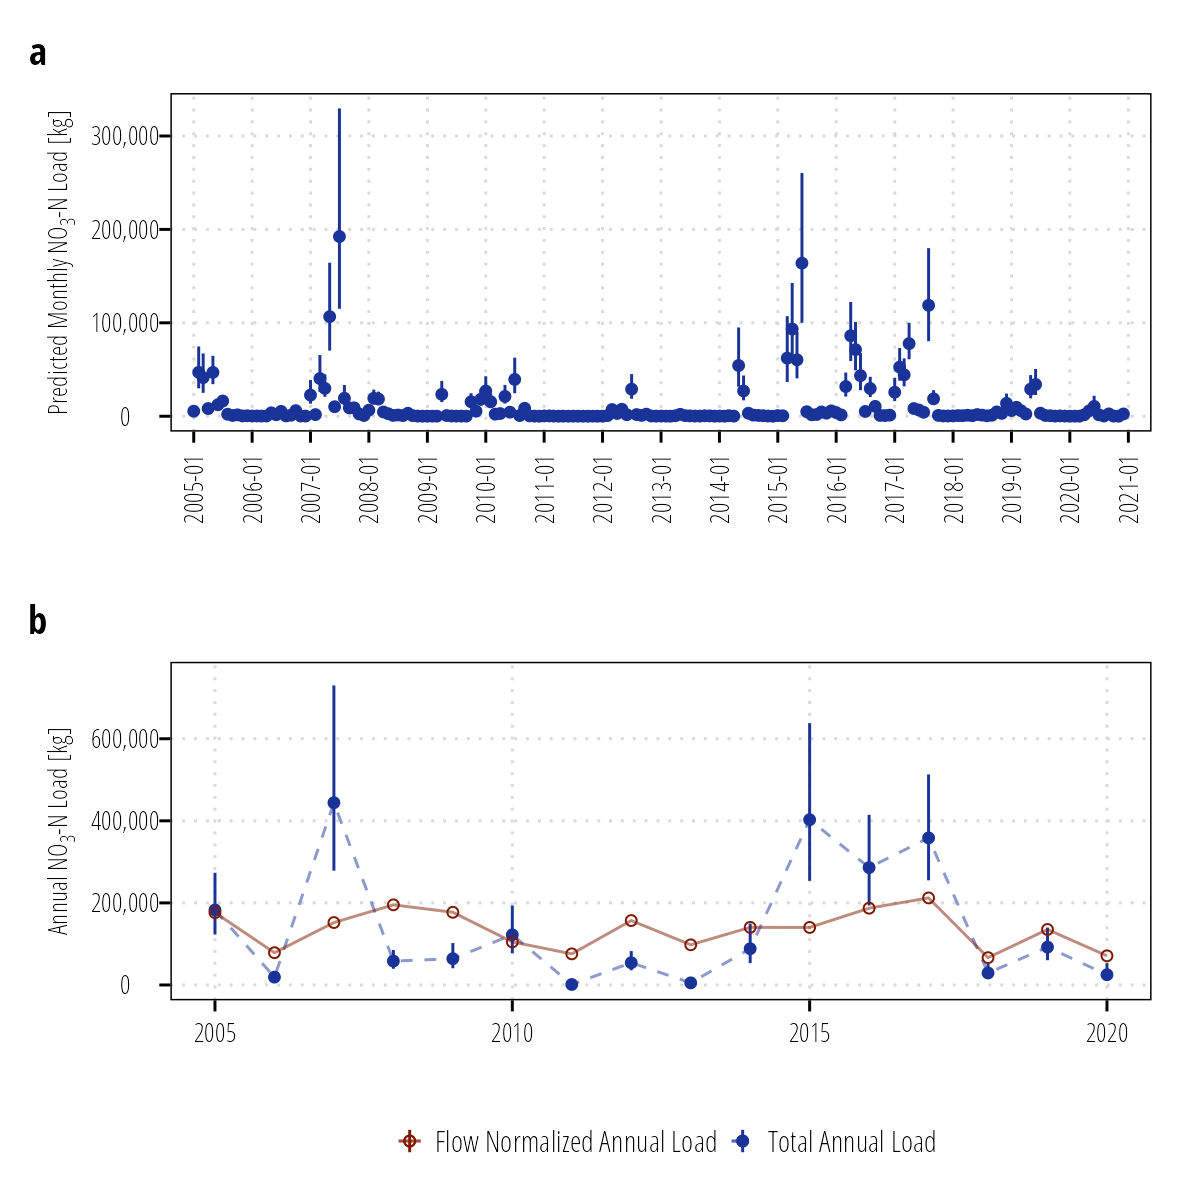
\includegraphics{load_estimates_files/figure-pdf/no3_aggregate-texana-1.png}

}

\caption{Aggregated (a) monthly and (b) annual NO\textsubscript{3}-N
loads at Palmetto Bend Dam at Lake Texana.}

\end{figure}

\begin{figure}[h]

{\centering 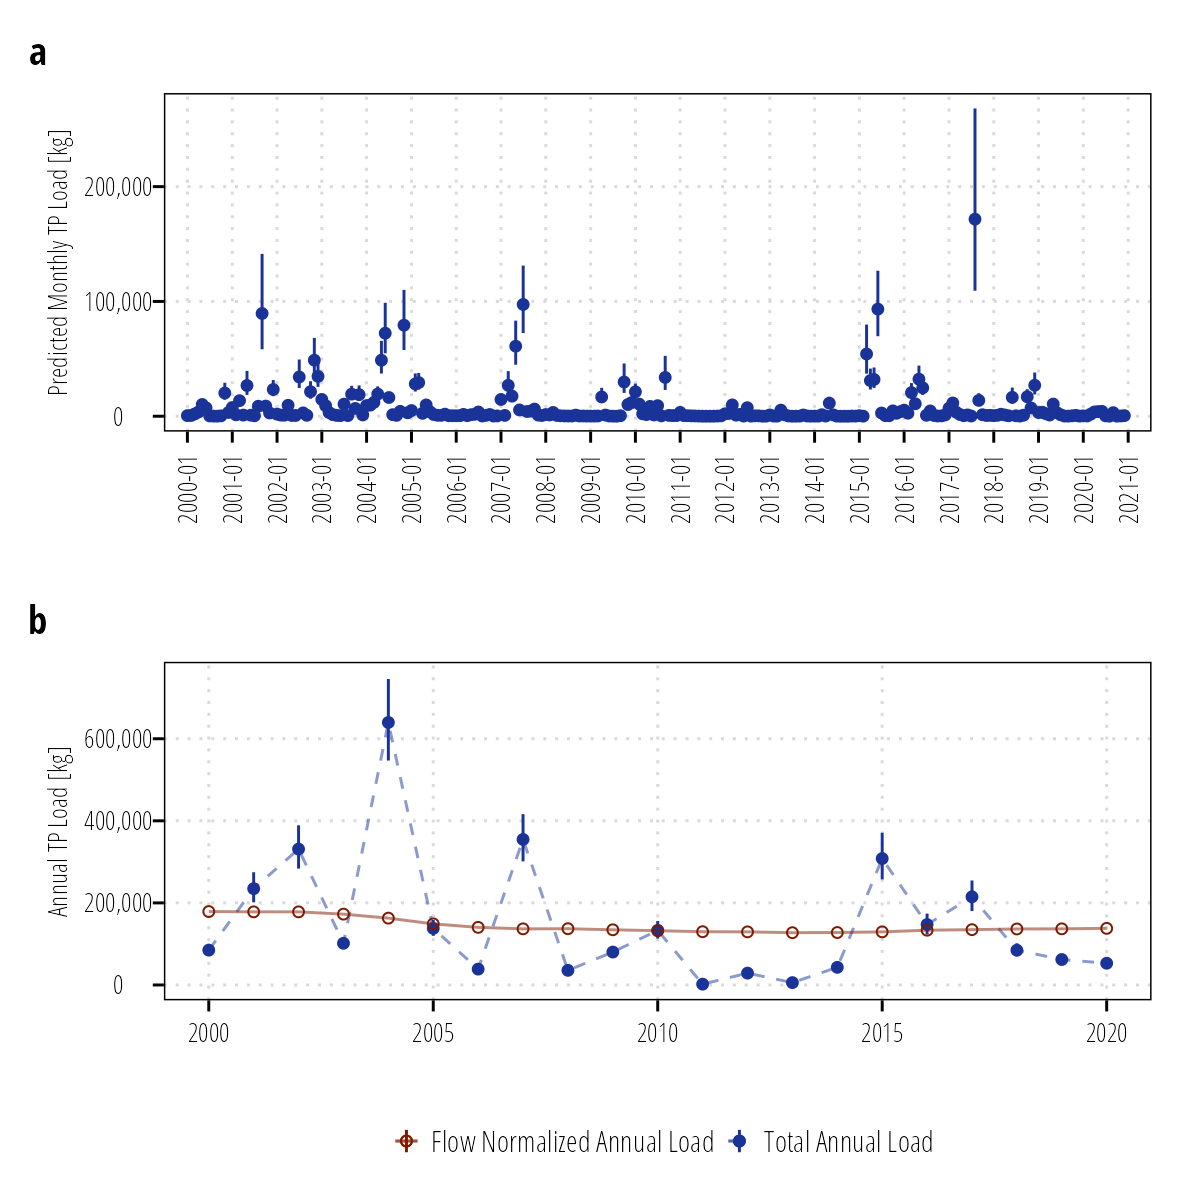
\includegraphics{load_estimates_files/figure-pdf/tp_aggregate-texana-1.png}

}

\caption{Aggregated (a) monthly and (b) annual TP loads at Palmetto Bend
Dam at Lake Texana.}

\end{figure}

\clearpage

\hypertarget{total-export}{%
\subsection{Total Export}\label{total-export}}

\hypertarget{no3-n}{%
\subsubsection{\texorpdfstring{NO\textsubscript{3}-N}{NO3-N}}\label{no3-n}}

\begin{figure}[h]

{\centering 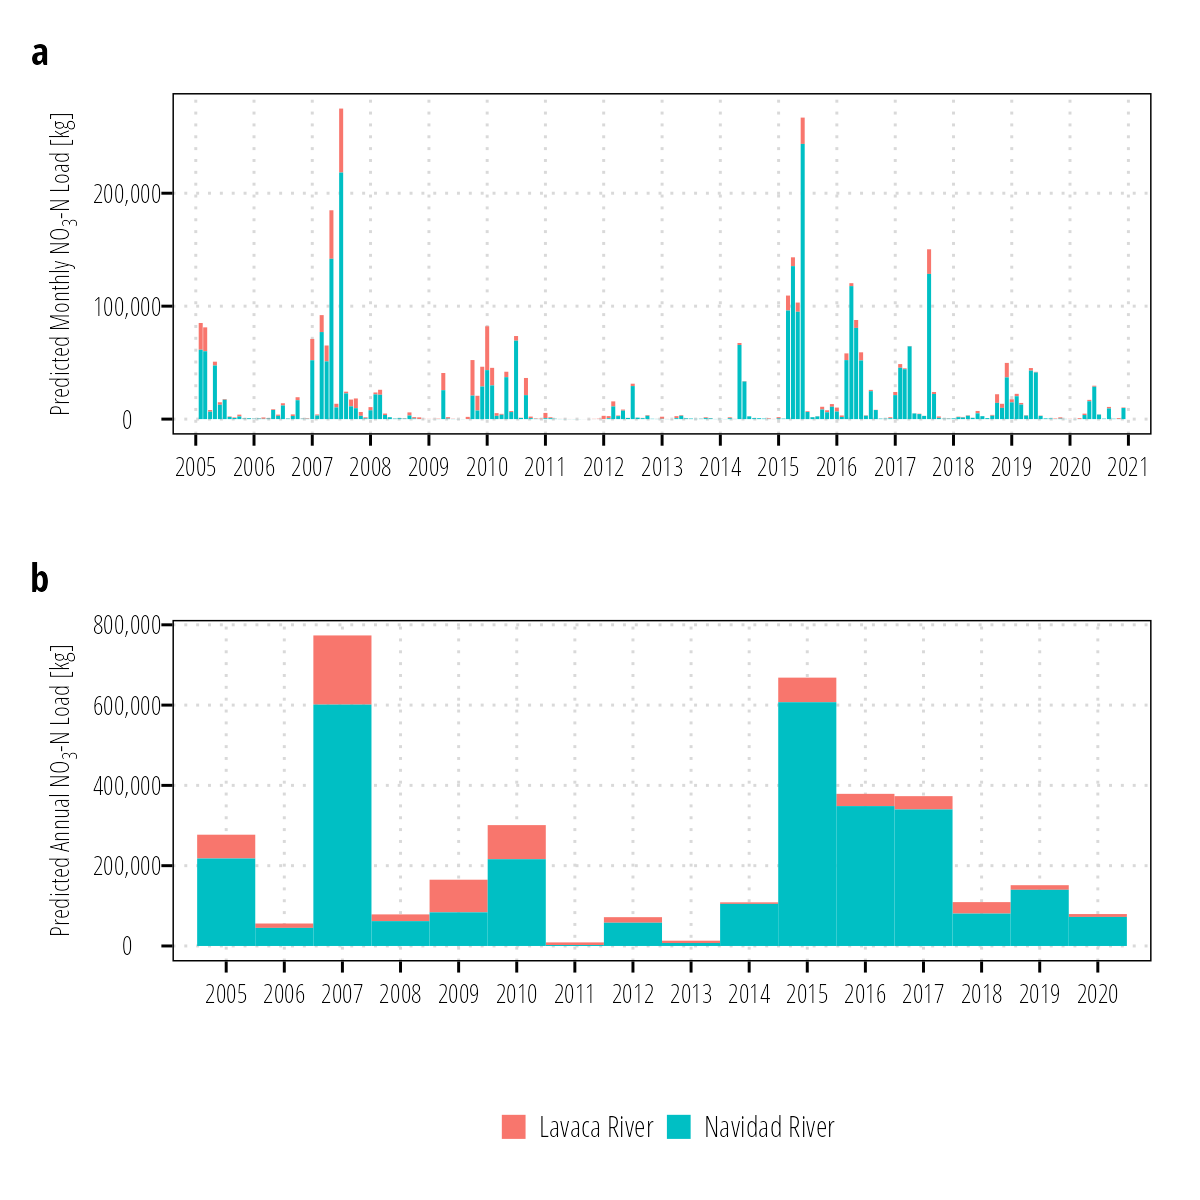
\includegraphics{load_estimates_files/figure-pdf/no3_total_export-1.png}

}

\caption{Modelled monthly and annual total NO\textsubscript{3}-N input
to Lavaca Bay}

\end{figure}

\clearpage

\hypertarget{tp}{%
\subsubsection{TP}\label{tp}}

\begin{figure}[h]

{\centering 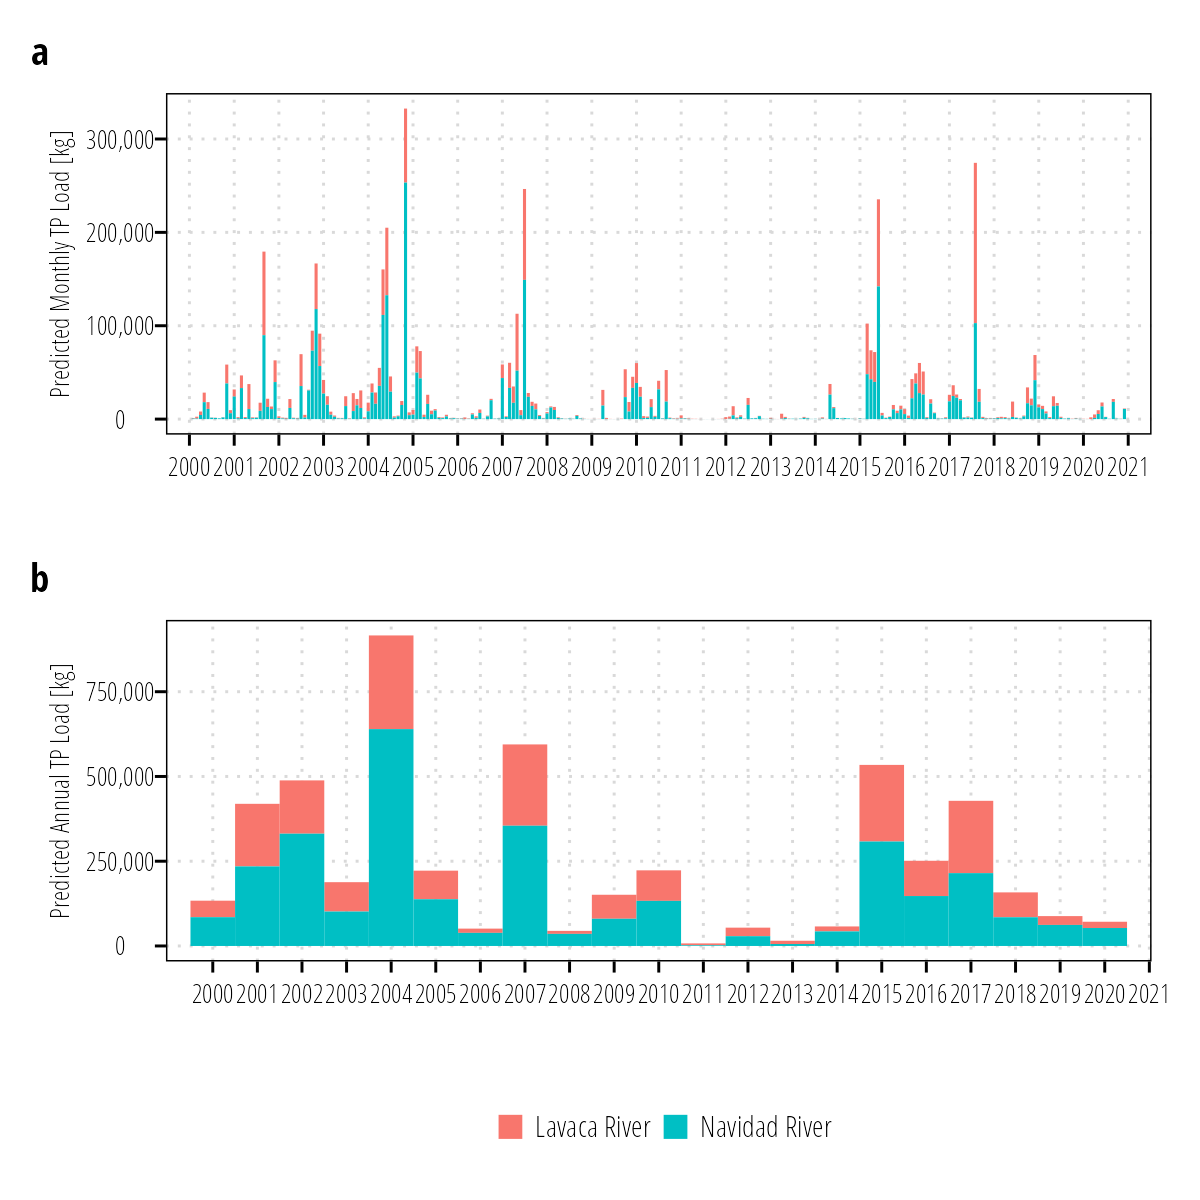
\includegraphics{load_estimates_files/figure-pdf/tp_total_export-1.png}

}

\caption{Modelled monthly and annual total TP input to Lavaca Bay}

\end{figure}

\clearpage

\hypertarget{references}{%
\section*{References}\label{references}}
\addcontentsline{toc}{section}{References}

\hypertarget{refs}{}
\begin{CSLReferences}{1}{0}
\leavevmode\vadjust pre{\hypertarget{ref-hirschWeightedRegressionsTime2010}{}}%
Hirsch, R.M., Moyer, D.L., and Archfield, S.A. 2010. Weighted
Regressions on Time, Discharge, and Season (WRTDS), with an Application
to Chesapeake Bay River Inputs1: Weighted Regressions on Time,
Discharge, and Season (WRTDS), With an Application to Chesapeake Bay
River Inputs. JAWRA Journal of the American Water Resources Association
46 (5): 857--80. \url{https://doi.org/10.1111/j.1752-1688.2010.00482.x}.

\leavevmode\vadjust pre{\hypertarget{ref-marraCoveragePropertiesConfidence2012}{}}%
Marra, G., and Wood, S.N. 2012. Coverage Properties of Confidence
Intervals for Generalized Additive Model Components: Coverage properties
of GAM intervals. Scandinavian Journal of Statistics 39 (1): 53--74.
\url{https://doi.org/10.1111/j.1467-9469.2011.00760.x}.

\leavevmode\vadjust pre{\hypertarget{ref-mcdowellImplicationsLagTimes2021}{}}%
McDowell, R.W., Simpson, Z.P., Ausseil, A.G., Etheridge, Z., and Law, R.
2021. The implications of lag times between nitrate leaching losses and
riverine loads for water quality policy. Scientific Reports 11 (1):
16450. \url{https://doi.org/10.1038/s41598-021-95302-1}.

\leavevmode\vadjust pre{\hypertarget{ref-woodCONFIDENCEINTERVALSGENERALIZED2006}{}}%
Wood, S.N. 2006. ON CONFIDENCE INTERVALS FOR GENERALIZED ADDITIVE MODELS
BASED ON PENALIZED REGRESSION SPLINES. Australian \& New Zealand Journal
of Statistics 48 (4): 445--64.
\url{https://doi.org/10.1111/j.1467-842X.2006.00450.x}.

\end{CSLReferences}



\end{document}
